\begin{savequote}[8cm]
A process cannot be understood by stopping it. Understanding must move with the flow of the process, must join it and flow with it. (First Law of Mentat)
  \qauthor{--- Frank Herbert, Dune}
\end{savequote}
%Edsger W. Dijkstra, How do we tell truths that might hurt? (1975).

\chapter{\label{ch:oxview_intro}An introduction to tools for the design and simulation of nucleic acid structures}

\minitoc

While previous chapters have covered modular self-assembly on a very abstract level, approximating the modules as simple cubes or patchy particles, this chapter will introduce tools and methods for designing and simulating individual structures or modules folded using DNA (or RNA).

The following sections will cover a selection of practical design and simulation tools that have been developed over the years, providing context for the presentation of my contributions to the \emph{oxView} tool in Chapter \ref{ch:oxview}.

% REFER TO THIS OVERVIEW!! https://pubmed.ncbi.nlm.nih.gov/33920889/


%Simulating the structure and dynamics of individual DNA origami modules has been possible for a while, but my aim with this project has been to make such simulations more accessible and easy to use and analyse.

%This is accomplished as I develop new tools and scripts while learning about the simulation methods and the designs that various laboratories are interested in.

%This chapter describes the currently available tools for simulation and design of individual module structures. DNA and RNA structures can be digitally represented in many different formats, for many different uses, and with different levels of coarse-graining. 

%The following sections cover my results over the last year, investigating methods for converting designs into the oxDNA/RNA format and for visualising and analysing the simulation results.

\section{Design tools}\label{sec:design_tools}
Designing a DNA origami structure by hand would be very laborious for anything but the most simple design. As such, a host of computer-aided design tools have been introduced over the years to make things easier. This section will cover some of the more common examples.

\subsection{Lattice-based design tools}
The caDNAno design tool \cite{cadnano} and the web-based scadnano\cite{scadnano} it inspired, allows the user to design DNA origami on a lattice of parallel helices.
\subsubsection{caDNAno}
\label{sec:cadnano}
CaDNAno \cite{cadnano} was introduced in 2009 as a way to simplify 2D and 3D DNA origami designs. It has a graphical user interface with multiple panels, seen in Figure \ref{fig:cadnano}. In the slice panel, the designer can place virtual helices on a lattice (either hexagonal or square), seen in the leftmost panel of the figure. The helices can then be filled in with strands and connected using crossovers in a path panel, seen in the middle of the figure.

Finally, caDNAno is also available as a plugin to the Autodesk Maya software, which enables a 3D visualisation of the design as seen in the render panel to the right in Figure \ref{fig:cadnano}. However, caDNAno does not support Maya versions after 2015 \cite{cadnanoInstall}.

\begin{figure}[h]
  \begin{center}
    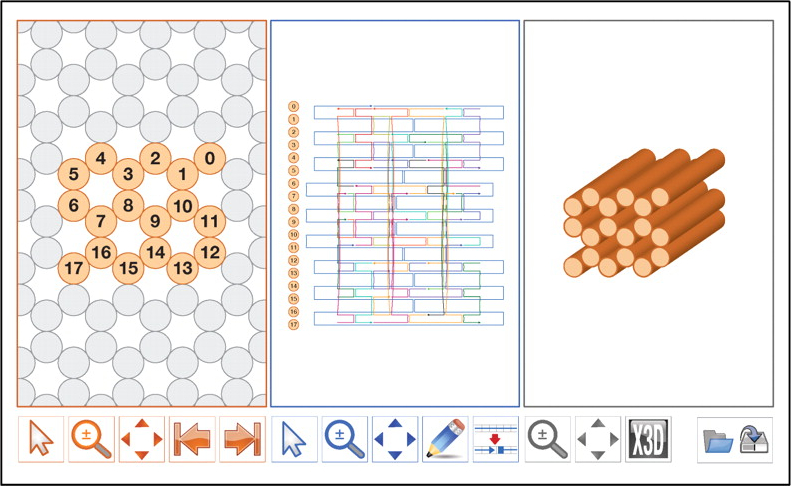
\includegraphics[width=\textwidth]{figures/cadnano.jpeg}
    \caption{The caDNAno design interface, adapted from figure 1.(a) in \cite{cadnano}}
    \label{fig:cadnano}
  \end{center}
\end{figure}

\subsubsection{Scadnano}
Scadnano \cite{scadnano} (scriptable caDNAno) is a relatively new design tool, independent from but inspired by caDNAno version 2. The main difference is that Scadnano is entirely web-based (thus not requiring any installation). The python code base is also designed to make it easier to write scripts generating DNA designs. Scadnano can be found at \url{https://scadnano.org/}.

\subsection{Top-down shape converters}
While tools like caDNAno simplify bottoms-up design, where the user builds structures from individual strands and nucleotides, a top-down tool can take a polyhedral target shape as input and provide a suitable origami design as output. 

% Mention DNA bricks software?

\subsubsection{BSCOR}\label{sec:bscor}
%https://doi.org/10.1038/nature14586

In 2015, Benson et al. published a method for converting arbitrary mesh designs into a DNA origami mesh \cite{vHelix}. Figure \ref{fig:bscor} shows a set of example polyhedral shapes, with the designed shape in a), the output DNA design in b), and microscopy characterisations in c)-d). A follow-up paper in 2016 also introduced the ability to design flat-sheet meshes \cite{benson2016computer}. BSCOR uses single DNA duplex edges, with double edges added whenever topologically necessary.

\begin{figure}[h]
  \begin{center}
    \includegraphics[width=\textwidth]{figures/bscor.png}
    \caption{3D meshes rendered in DNA origami using BSCOR. Adapted from \cite{vHelix}.}
    \label{fig:bscor}
  \end{center}
\end{figure}


\subsubsection{ATHENA}
% DAEDAULS/PERDIX
%https://www.science.org/doi/full/10.1126/science.aaf4388
 %ATHENA? https://academic.oup.com/nar/advance-article/doi/10.1093/nar/gkab762/6368527 - Use fig 2 in now published paper!!!

 ATHENA is a recently published tool for automatic design wireframe origami shapes. As seen in Figure \ref{fig:athena}, earlier software such as PERDIX, METIS, DAEDAULS and TALOS have facilitated design for 2D and 3D wireframes respectively, using different edge designs, but ATHENA aims to bring them all toghether as a single package.


\begin{figure}[h]
  \begin{center}
    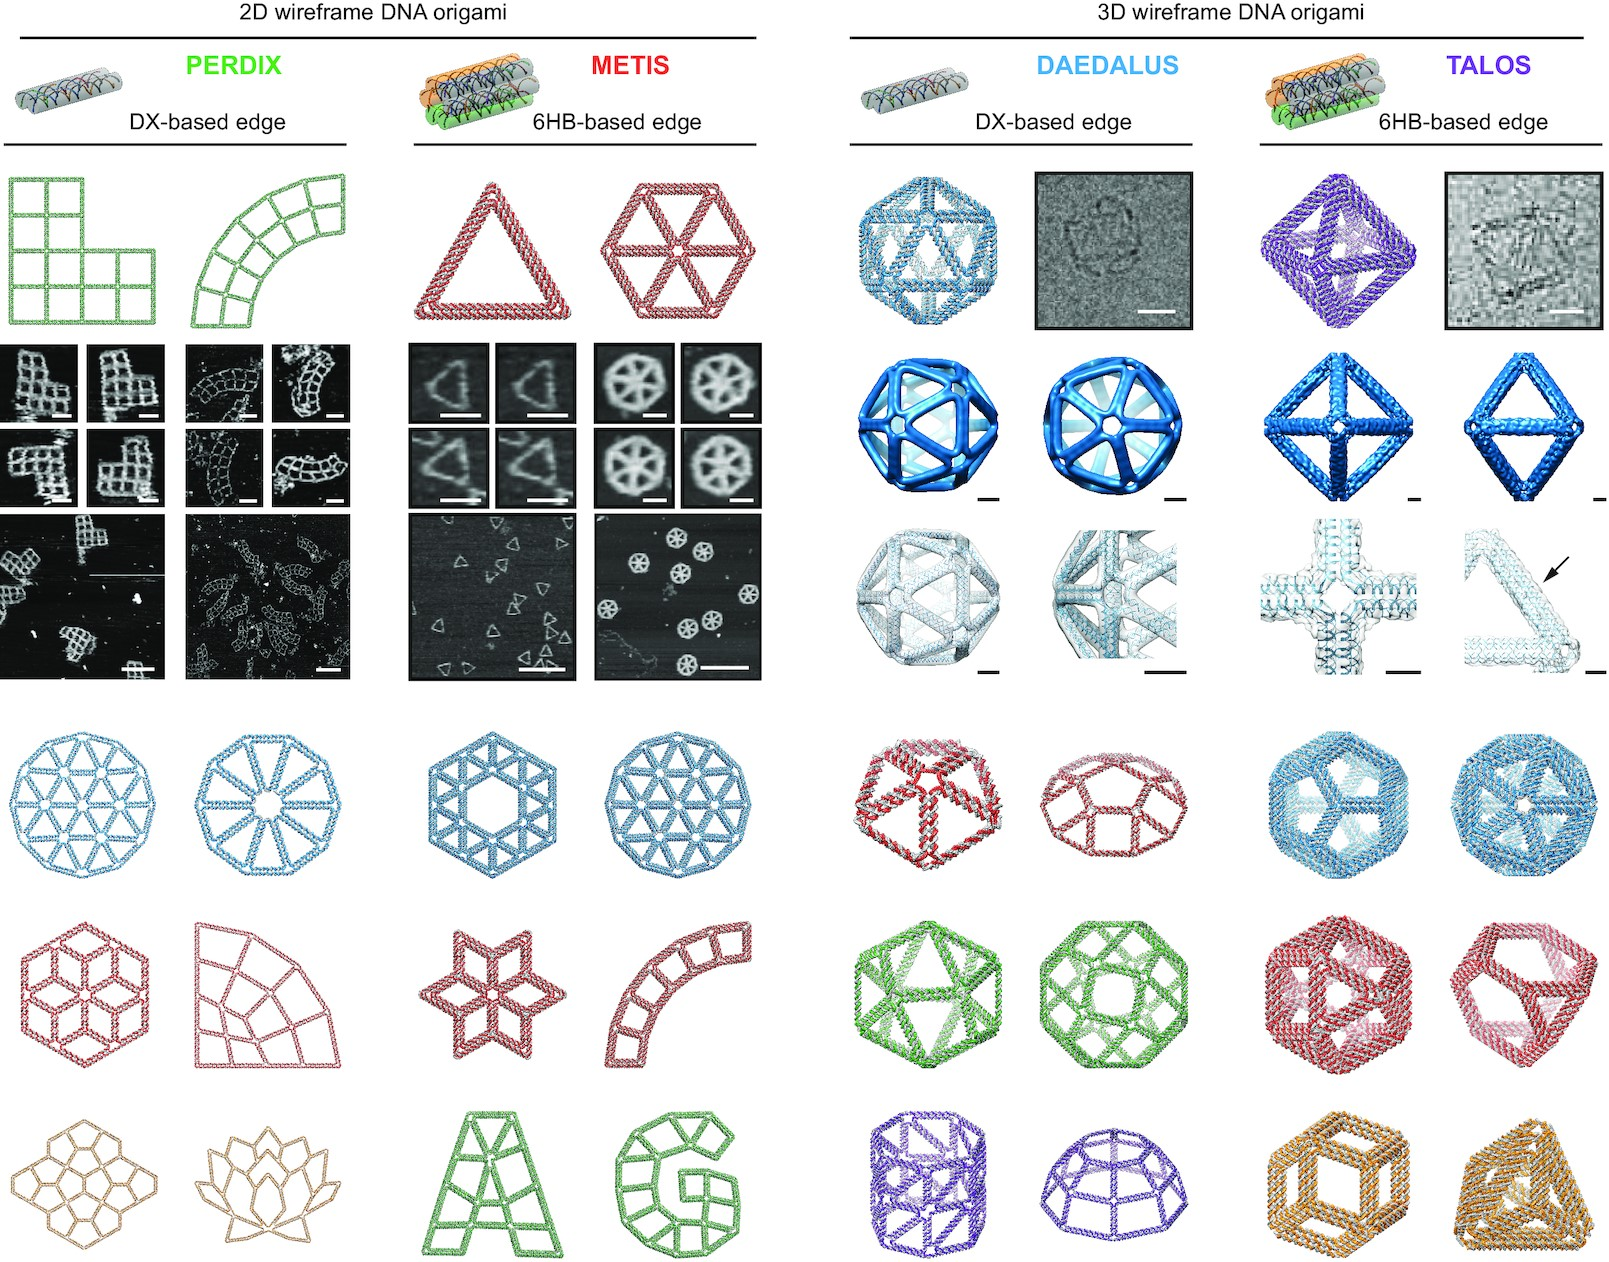
\includegraphics[width=\textwidth]{figures/athena.jpeg}
    \caption{Automatic wireframe origami shapes using ATHENA. Adapted from \cite{athena}. }
    \label{fig:athena}
  \end{center}
\end{figure}

\subsubsection{Triangulated truss structures}
% M. Matthies
% https://pubs.acs.org/doi/abs/10.1021/acs.nanolett.6b00381

\subsection{Free-form or hybrid tools}

\subsubsection{Tiamat}
Tiamat is an early free-form design tool introduced in 2009.

\begin{figure}[h]
  \begin{center}
    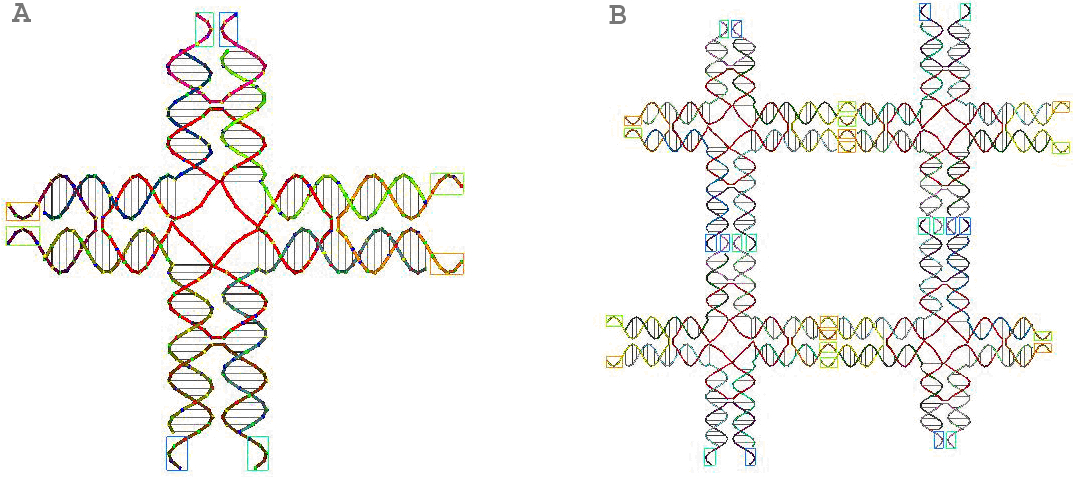
\includegraphics[width=\textwidth]{figures/tiamat.png}
    \caption{Tiamat}
    \label{fig:tiamat}
  \end{center}
\end{figure}

\subsubsection{vHelix}

\begin{figure}[h]
  \begin{center}
    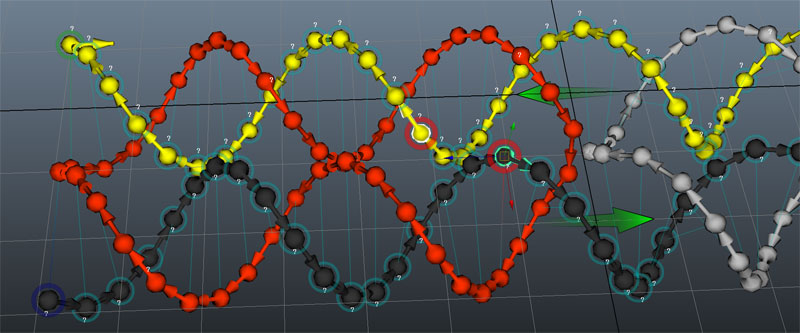
\includegraphics[width=\textwidth]{figures/vhelix.jpg}
    \caption{vHelix}
    \label{fig:vhelix}
  \end{center}
\end{figure}


\subsubsection{Adenita}
Adenita \cite{miao_tvcg_2018} is a free-form editing tool developed as a plugin to the SAMSON toolkitb


\begin{figure}[h]
  \begin{center}
    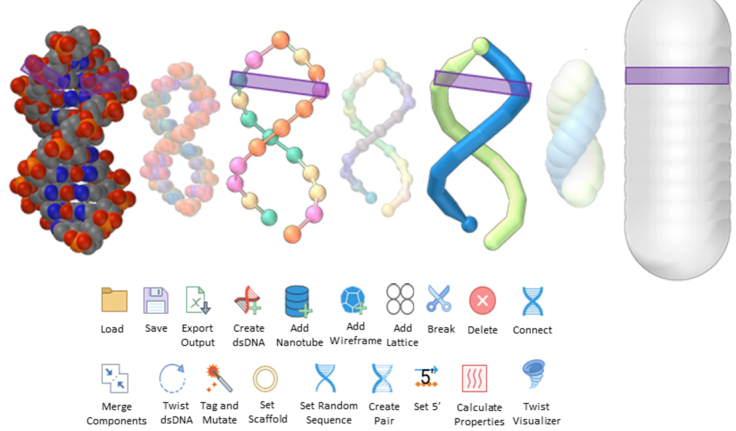
\includegraphics[width=\textwidth]{figures/adenita.jpg}
    \caption{Adenita}
    \label{fig:adenita}
  \end{center}
\end{figure}

\subsubsection{MagicDNA}
Another method of solving topological issues through rigid-body manipulation was used by Chao-Min Huang \cite{huang2021integrated}. MagicDNA, as seen in Figure \ref{fig:magicDNA}, has an computer-aided design workflow where geometry can be specified from helix cross-sections or imported from a part library, then assembled into an integrated structure (using multiple scaffolds if neccesary).

MagicDNA is written as a plugin to the Matlab suite.


\begin{figure}[h]
  \begin{center}
    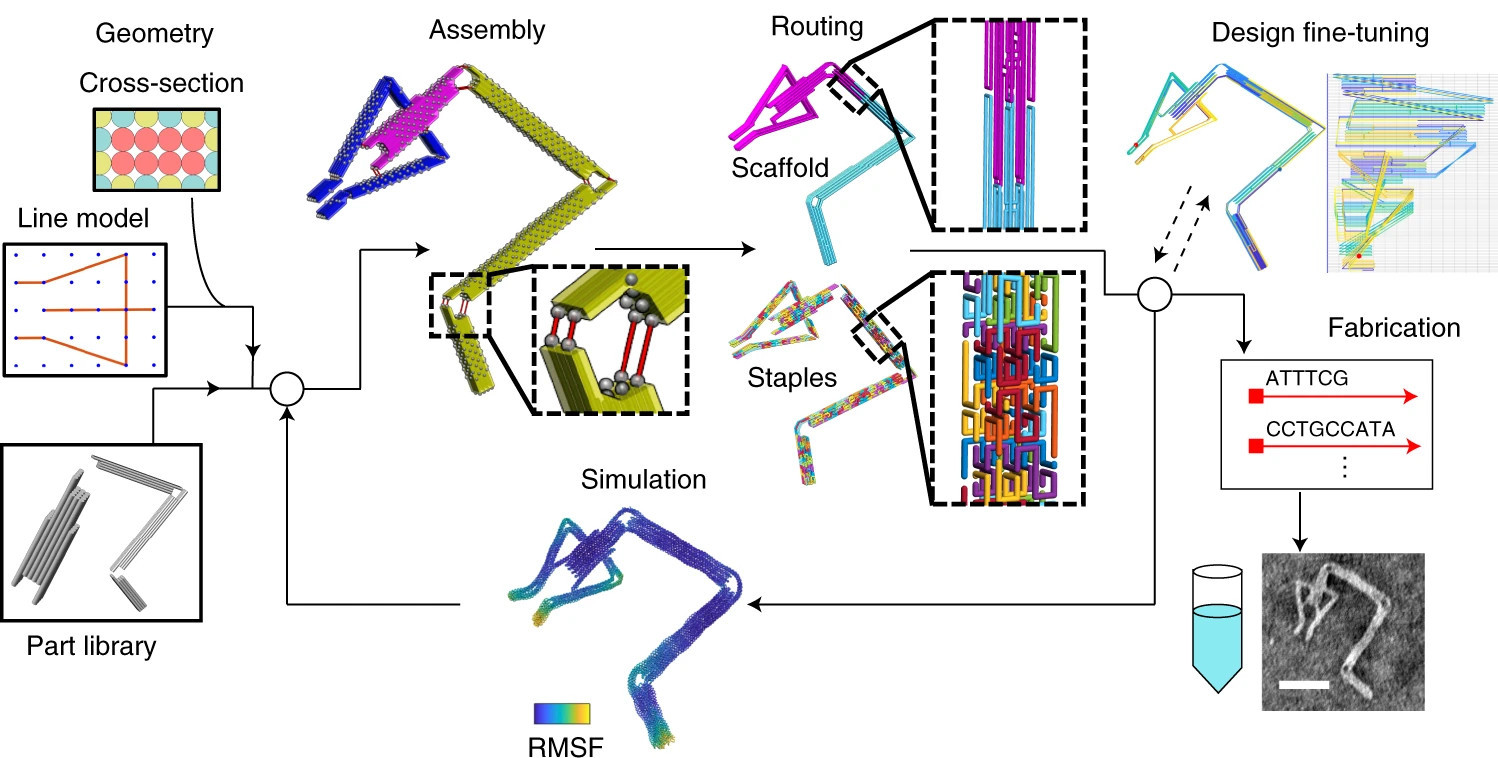
\includegraphics[width=\textwidth]{figures/magicDNA.jpeg}
    \caption{MagicDNA adapted from \cite{huang2021integrated}.}
    \label{fig:magicDNA}
  \end{center}
\end{figure}

\subsubsection{oxView}
The oxView application was developed as part of this thesis project and will be described more in Chapter \ref{ch:oxview}.

\section{Simulation tools}
Simulating a structure can provide insight to understand experimental results but can also guide decisions at the design stage. Different models

\subsection{All-atom simulation}
Simulation tools such as NAMD\cite{NAMDphillips2005scalable}, use force fields such as AMBER\cite{AMBERcornell1996second} and CHARMM \cite{brooks1983charmm} that model interactions between individual atoms. While it is possible to perform atomistic simulations of large DNA origami structures\cite{yoo2013situ}, the simulations take a long time to run, and it is unknown how well the models represent DNA thermodynamics \cite{sengar2021primer}.

%Also cite Pointer origami https://academic.oup.com/nar/article/44/7/3013/2467847 ?

\begin{figure}[h]
  \begin{center}
    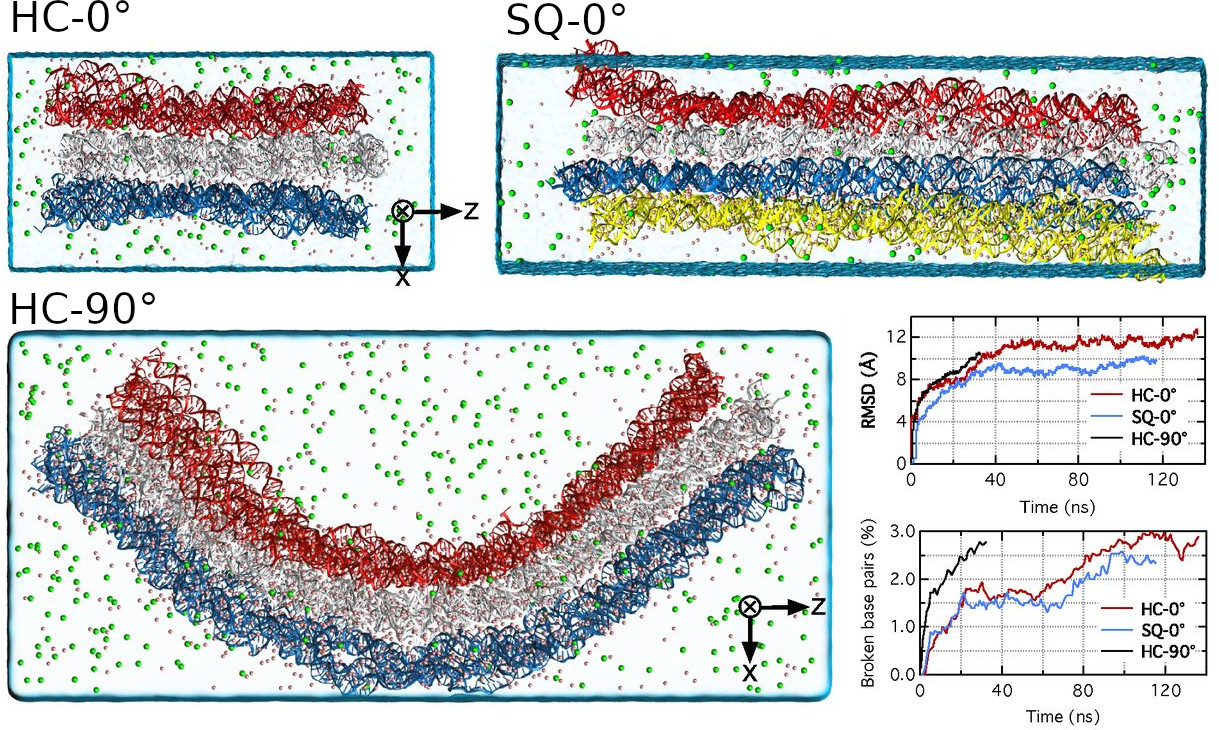
\includegraphics[width=\textwidth]{figures/all-atom.jpg}
    \caption{All-atom simulation}
    \label{fig:all-atom}
  \end{center}
\end{figure}

\subsection{oxDNA/RNA}
In 2010, a coarse-grained simulation software called oxDNA was introduced by Thomas Ouldridge \cite{ouldridge2010dna}. It simulates DNA on the level of nucleotides and has been shown to model complex origami devices with a generally good agreement with experimental data \cite{sharma2017characterizing}. In 2014, the DNA model was extended to include RNA by Petr {\v{S}}ulc \cite{vsulc2014nucleotide}, showing its ability to model a set of common RNA motifs. 

Molecular Dynamics (MD) and Monte Carlo (MC) simulation techiniques.

OxDNA was joined by cogli1 for trajectory visualisation.


% Mention ANM model by Jonah!!!

While oxDNA can be very useful for modelling a structure, it has traditionally not been very accessible for experimentalists. % mention web server

\begin{figure}[h]
\begin{center}
    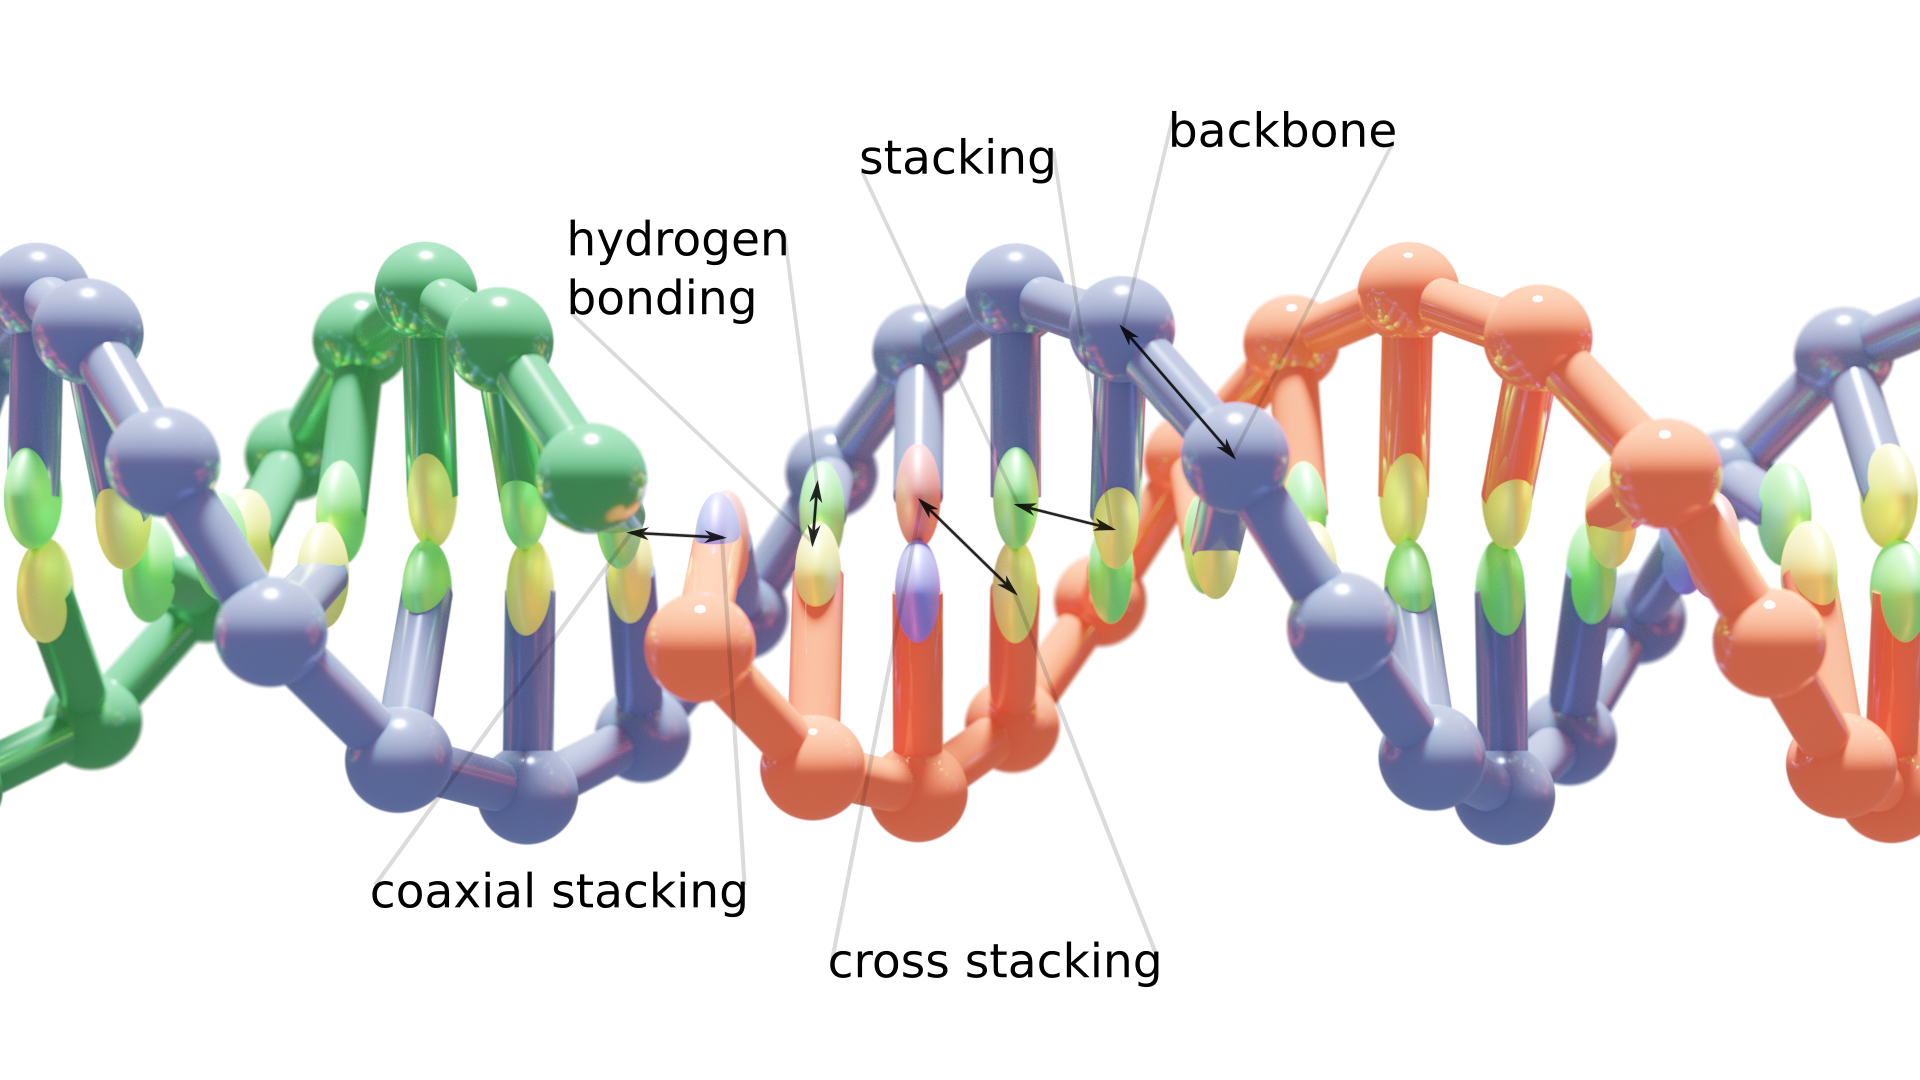
\includegraphics[width=\textwidth]{figures/oxdna_annot.png}
    \caption{The oxDNA model}
    \label{fig_oxDNA}
    \end{center}
\end{figure}

\subsection{mrDNA}
Another promising feature of mrdna is that it has a spline-based helix representation and is implemented in python. This enables users to easily script edits to the structure, translating and rotating parts of it before starting the simulation. Thus, topological issues or over-stretched bonds can, with some skill, be resolved even before starting to simulate. I did, based on this, also create a rudimentary interactive editor interface to mrdna, but it would need a lot of refinement to be externally usable.

\begin{figure}[h]
  \begin{center}
    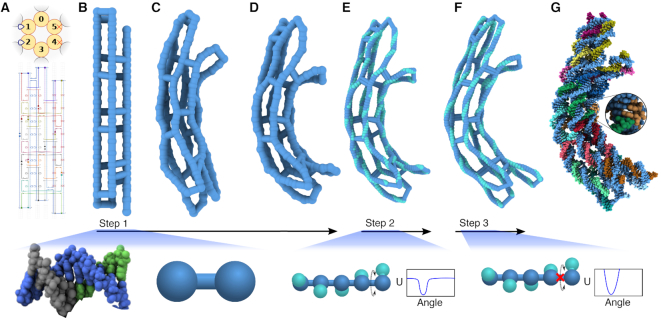
\includegraphics[width=\textwidth]{figures/mrDNA.jpg}
    \caption{MrDNA}
    \label{fig:mrdna}
  \end{center}
\end{figure}

A selection of the DNA designs I have relaxed are shown in Figure \ref{fig:oxDNA_sims}. The first two examples, adopted from \cite{gerling2015dynamic} and \cite{zadegan2012smallbox} and illustrated in Figure \ref{fig:oxDNA_sims}.a and \ref{fig:oxDNA_sims}.b, are both quite straightforward to relax in oxDNA, although the relaxation is much faster using mrdna.

The tensegrity kite structure, adopted from \cite{liedl2010_kite} is harder to relax since, as seen in the first image in Figure \ref{fig:oxDNA_sims}.c, the two helix bundles are drawn parallel to each other in caDNAno. Given enough time to relax, they should still become orthogonal, but a much more efficient way is to write a mrdna script to rotate one helix bundle so that it is orthogonal from the start, as seen in the middle image of \ref{fig:oxDNA_sims}.c. The remaining overstretched bonds are then quickly relaxed using mrdna.

Finally, the Möbius strip, adopted from \cite{han2010moebius}, is particularly tricky to relax, since the caDNAno design have all helices drawn in the same plane, with bonds from each end stretching through the whole structure and intersecting at a single point, as can be seen in the first image of Figure \ref{fig:oxDNA_sims}.d. With some help from Chris Maffeo, however, I was able to use a mrdna script to edit the structure into a configuration much easier to relax, as seen in the second image of Figure \ref{fig:oxDNA_sims}.d. Since the caDNAno design does not make it clear if the Möbius strip should be left-handed or right-handed, this is also decided in the script; changing the rotational direction will produce a mirrored version of the structure, as seen in the third image of Figure \ref{fig:oxDNA_sims}.d.

\begin{figure}
  \centering
  \begin{overpic}[width=\textwidth]{figures/oxdna_sims.eps}
    \put(0,960){a)}
    \put(0,760){b)}
    \put(0,540){c)}
    \put(0,260){d)}
  \end{overpic}
  \caption{Relaxation results for various DNA designs. Each row depicts a new design, with the left-hand side showing the structure as it was drawn in caDNAno (and parsed by mrdna), while the right-hand side is the relaxed structure in oxDNA. Intermediate images are edits done in mrdna. While the switch design\cite{gerling2015dynamic} in \textbf{a)} 
  and the small DNA origami box\cite{zadegan2012smallbox} in \textbf{b)} relaxed without any required editing, the tensegrity kite structure \cite{liedl2010_kite} in \textbf{c)} and the Möbius strip\cite{han2010moebius} in \textbf{d)} benefited greatly from moving selected helices to a position off the lattice before starting the simulation.}
  \label{fig:oxDNA_sims}
\end{figure}

\subsection{Cando}

Cando is a finite element modelling framework\cite{kim2012cando} available through a web server at \url{https://cando-dna-origami.org}. DNA double helices are modelled as elastic rods (connected by rigid crossovers) that stretch, twist and bend in line with experimental measurements.

\begin{figure}[h]
  \begin{center}
    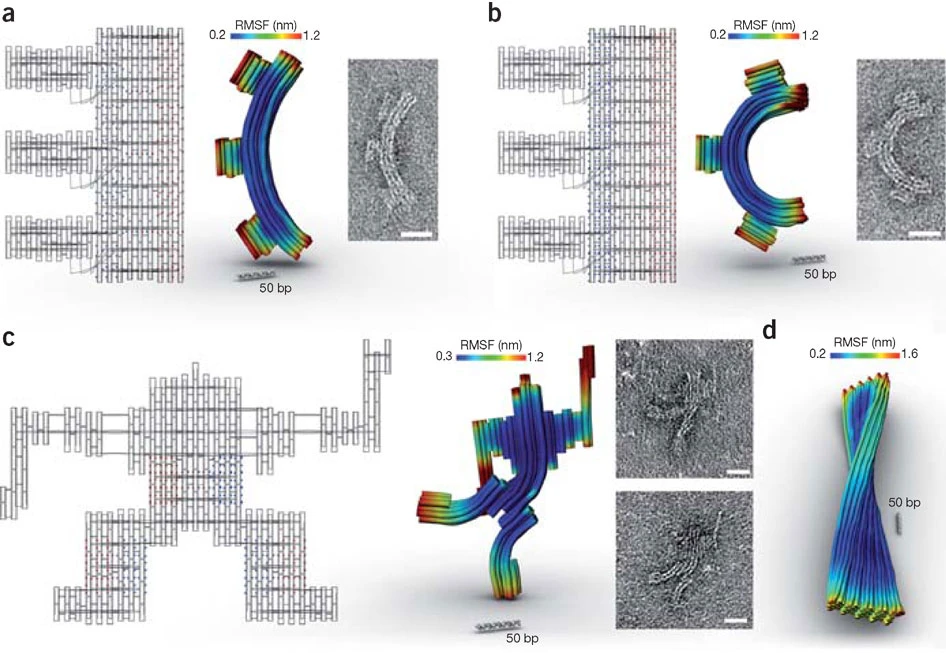
\includegraphics[width=\textwidth]{figures/cando.png}
    \caption{Cando}
    \label{fig:cando}
  \end{center}
\end{figure}